%!TEX TS-program = lualatex
%!TEX encoding = UTF-8 Unicode
\RequirePackage{luatex85}
\RequirePackage{shellesc}
\documentclass[12pt,oneside]{article}
\usepackage{geometry}
	\geometry{a4paper,bottom=5cm}

\usepackage[usenames,dvipsnames]{xcolor}
   \definecolor{UOWred}{RGB}{245, 15, 20}%
   \definecolor{UOWblue}{RGB}{0, 51, 204}% {cmyk}{90, 68, 0, 0} % 
   \definecolor{UOWdarkblue}{RGB}{12, 35, 64}% {cmyk}{100, 76, 12, 70} % 

\usepackage[explicit]{titlesec}
    \titleformat{\section}
        {\color{Blue}\normalfont\Large\sffamily}
        {\color{Blue}\thesection}{1em}{\allcaps{#1}}
    \titleformat{\subsection}
        {\normalfont\large\sffamily}
        {\thesection}{1em}{#1}
        
\usepackage[scale=2]{ccicons}
\usepackage{fontspec,xltxtra} 
\defaultfontfeatures{Mapping=tex-text}
  \setromanfont[Numbers=OldStyle]{Times LT Std}
  \setsansfont[Scale=MatchLowercase]{Montserrat}
  \setmonofont[Scale=MatchLowercase]{Menlo}
  
\usepackage[tracking=true,protrusion=true,expansion=true]{microtype}
  \DeclareMicrotypeSet*[tracking]{my}{%
        encoding = *,%
        % size     = {-small,Large-},%
        size     = {,Large-},%
        font     = */*/*/sc/*,%
     }
  \SetTracking{ encoding = *, size = -small }{ 20 }
  \SetTracking{ encoding = *, size = Large- }{ -20 }
  \SetTracking[ no ligatures = {f,t} ]{ encoding = *, shape = {sc*},}{60}
  \newcommand{\allcapsspacing}[1]{\textls*[40]{#1}}%
  \newcommand{\allcaps}[1]{\allcapsspacing{\MakeTextUppercase{#1}}}%

\usepackage{textcase}
\usepackage{embrac}
\usepackage{pdfpages}
\usepackage{hyperref}

\usepackage{listings}
  \lstset{%
    % language=[LaTeX]TeX,%
    basicstyle=\footnotesize\ttfamily,%
    breakatwhitespace=false,%
    keepspaces=true,%
    % keywordstyle=\color{UOWred},%
    % texcsstyle=\color{UOWred},%
    % morekeywords={%
    %   \,%
    %   \{,%
    %   \},%
    %   \[,%
    %   \],%
    %   begin,%
    %   textcopyright,%
    %   vspace,%
    %   smallgap,%
    %   RTPacknowledgement,%
    %   ifdomestic%
    % },%
    numbers=left,%
    numbersep=5pt,%
    numberstyle=\tiny,%
  }


\makeatletter
\renewcommand*\l@section{\@dottedtocline{1}{1.5em}{2.3em}} % dots in the table of contents
\makeatother

\newcommand{\option}[1]{\texttt{\color{UOWblue}#1}} 
% simplified the highlighting of options and commands in text
\newcommand{\command}[1]{\texttt{\color{UOWred}#1}} 
% simplified the highlighting of options and commands in text
\newcommand{\comoptions}[1]{\texttt{\color{UOWdarkblue}#1}} 
% simplified the highlighting of options and commands in text

\setcounter{secnumdepth}{0}

\begin{document}
    
\title{\textsf{uowthesistitlepage}}
\author{\small Thomas M. Griffiths}
\date{Released \today, Version 3.0}

\maketitle

\tableofcontents

\section{About}
This package redefines the \command{\textbackslash{}maketitle} command to generate a title page compliant with the University of Wollongong (\textsc{uow}) branding guidelines. A copyright declaration is printed on the page immediately following the title page, including the required acknowledgement of the Australian Government Research Training Program Scholarship. This package also defines a command, \command{\textbackslash{}declaration}, which typesets a declaration page, required in the front matter of each PhD thesis. 

The package has a number of options that change the wording of the title page according to whether your thesis is only one part of, or comprises the entire of assessable component for your degree and the number of supervisors you have (if any). The default when the package is loaded is an \option{honours} thesis.

This package \emph{is not} a complete thesis template or document class, it \emph{only} typesets the title page and declaration. This package is designed to do as little to your document as possible. It won't set the margins, spacing, or typeface used in your document. There is a template document online that you can download. It follows the \textsc{uow} thesis guidelines and is has a basic setup ready to get you started with your thesis. For those starting off on their own, the following code will give you a document that satisfies the \textsc{uow} thesis guidelines.\\

\command{\textbackslash{}documentclass}\option{[twoside,12pt,a4paper]}\comoptions{\{book\}}

\command{\textbackslash{}usepackage}\comoptions{\{geometry\}}

\command{\textbackslash{}geometry}\comoptions{\{a4paper,inner=4.0cm, outer=2cm, top=3cm, bottom=2cm\}}

\command{\textbackslash{}usepackage}\comoptions{\{setspace\}}

\command{\textbackslash{}onehalfspacing}

\texttt{\% or}

\texttt{\%} \command{\textbackslash{}doublespacing}

\texttt{\% to use in Times New Roman instead of the LaTeX default, latin modern.}

\command{\textbackslash{}usepackage}\comoptions{\{mathptmx\}}


\section{Usage}
\subsection*{\command{\textbackslash{}maketitle}}
If you are familiar with \LaTeX{} using this package is very simple, place the package in your document's preamble:\\

\command{\textbackslash{}usepackage}\option{[options]}\comoptions{\{uowthesistitlepage\}}\\

\noindent The standard parts of the \command{\textbackslash{}maketitle} command still apply. The title, author and date fields are filled in as normal.\\

\command{\textbackslash{}title}\comoptions{\{A Pretty Swish Title\}}

\command{\textbackslash{}author}\comoptions{\{Average J. Blow\}}

\command{\textbackslash{}date}\comoptions{\{Month Year\}}\\

The new fields from the uowthesistitlepage package are\command{\textbackslash{}degree}, \command{\textbackslash{}school} and \command{\textbackslash{}supervisor} and the optional \command{\textbackslash{}cosupervisor}. They're fairly self-explanatory, and you use them just as you would the standard macros for the regular \command{\textbackslash{}maketitle} command.\\
  
\command{\textbackslash{}degree}\comoptions{\{That Degree You've Been Studying\}}
 
\command{\textbackslash{}school}\comoptions{\{Your School\}}

\command{\textbackslash{}supervisor}\option{[x]}\comoptions{\{Supervisor 1, Supervisor 2,\ldots{} \textbackslash{}\& Supervisor x\}}\\

You need to ensure a copy of the logo named \texttt{uow\textunderscore{}logo} is in the working directory where you're compiling your thesis.\footnote{Unless you're using the \option{report}, \option{fullsubject} or \option{partialsubject} options. These title pages have have no logo.} If you downloaded this style from the \textsc{uow} website there will be one in the zipped package. When you want to typeset the title page simply use \command{\textbackslash{}maketitle} after \command{\textbackslash{}begin}\comoptions{\{document\}} as you usually would.

\subsection*{\command{\textbackslash{}declaration}}
The declaration page is intended for PhD theses, but will work fine for each document type. Using the \command{\textbackslash{}declaration} command is simple, just place it in your document where you want it typeset. 

As of 2017, the package also typesets the copyright declaration for your thesis on the page immediately following the title page. This is the next page in one-sided documents, While in two-sided documents this will be the reverse of the title page. The copyright statement also contains the required acknowledgement of the Australian Government Research Training Program Scholarship as specified by the graduate research school. This is \emph{required} for domestic students. International students can use the \option{international} option to the package to print the copyright statement without the scholarship acknowledgement. There is also a macro to define your own copyright text should you require. And if you desire no copyright text at all then you can use the \option{nocopyright} option. 


\section{Package Options and Macros}
\subsection*{Macros}
\begin{description}
    \item[\command{\textbackslash{}author}\comoptions{\{Your Name\}}]
    The author of the work, in this case you. For the your thesis you should use your full name and any previous degrees, for example: Average Joe Blogs BSc Hon.
    
    \item[\command{\textbackslash{}subject}\comoptions{\{Your Subject\}}] If this is a dissertation submitted for an individual subject instead of a whole degree this is where you tell the package what it is. You can write the subject code, e.g. CHEM364, or the full subject name: `CHEM364, Molecular Structure and Spectroscopy'. If you're using this command you need to have the \option{report}, \option{fullsubject} or \option{partialsubject} option loaded in the preamble. If you don't load one of these three options this macro will do a disappointing nothing.
    
    \item[\command{\textbackslash{}cosupervisor}\option{[number of co-supervisors]}\comoptions{\{Your Co-supervisors\}}] This field is optional for your title page. It prints your co-super\-visor(s) to the title page. List all your co-supervisors and their titles in the one set of enclosing braces (\comoptions{\{~\}}), separated by commas and `and' or an ampersand (\textbackslash{}\&) before the final co-supervisor if you have multiple supervisors. Use the optional argument `\option{[x]}' to specify how many co-supervisors you have.
    
    This field can be modified to either display adjacent to the supervisor field or below it. Making the fields adjacent is done with the \option{horizontal} option in the preamble. The default is below the supervisor field. If you have a large number of supervisors, or supervisors with long names I recommend you use the default one above the other placing of the supervisor and co-supervisor fields.
    
    \item[\command{\textbackslash{}date}\comoptions{\{Month Year\}}] The date of your submission, usually `Month Year'. Alternatively, you can use the \command{\textbackslash{}today} macro, and it will print the date in the format month dd, yyyy.
    
    \item[\command{\textbackslash{}declaration}] The declaration is generally required in the front matter of a PhD thesis, and so the declaration page is mainly intended for PhD theses, but can also be used for all the other document types. The package will adjust the wording accordingly each document type; `report' for reports, `dissertation' for subject based documents (the declaration for these documents will also mention that they were submitted for a class, not the conferral of a degree) and `thesis' for all postgraduate work. It's used in the exact same way as \command{\textbackslash{}maketitle}, place it in the document where you want it typeset and it will typeset the following for example, for a PhD:\\
    
\noindent{\large \textbf{Declaration}}\\

{\noindent I, \emph{Student's Full Name}, declare that this thesis submitted in fulfilment of the requirements for the conferral of the degree \emph{Doctor of Philosophy}, from the University of Wollongong, is wholly my own work unless otherwise referenced or acknowledged. This document has not been submitted for qualifications at any other academic institution.\par
\vspace{1cm}
\noindent\rule{0.4\textwidth}{0.5pt}
\vspace{1ex}\\
\textbf{Student's Full Name}\\
\today}\\

    \item[\command{\textbackslash{}degree}\comoptions{\{Your Degree\}}] The degree for which you are submitting this work. Write the degree out in full; Doctor of Philosophy, Master of Science, Bachelor of Arts Honours etc.
    
    \item[\command{\textbackslash{}graphic}] This macro is used internally to load the \textsc{uow} Graphic. It has no immediate use in the body of your document and can be ignored unless you feel like cracking open the style file and tinkering. For the graphic to load properly in the title page there must be an image file in the working directory named \texttt{uow\textunderscore{}logo}. It can be used in the body of the document to load an alternative graphic if that is desired, be warned that determining the size in this case is up to you.
    The usage is a bit odd note the nested \command{\textbackslash{}includegraphics} command:
    
    \command{\textbackslash{}graphic}\comoptions{\{\textbackslash{}includegraphics\{yourgraphic\}\}}
    
    \item[\command{\textbackslash{}requirement}] Similar to the \command{\textbackslash{}graphic} macro, this macro is for internal use. It is manipulated by the degree options (\option{phd}, \option{honours} etc.) in the preamble, and determines what is printed in the requirement section of the title page.
    
    \item[\command{\textbackslash{}school}\comoptions{\{Your School\}}] The school within the university with which you are associated. If you are not associated with a school you can use the \option{noschool} option in the preamble to disable the school at the bottom of the title page. The \option{\textbackslash{}school} command will still work with the \option{noschool} option, so you can specify another affiliation, for example: The Australian Institute for Innovative Materials (AIIM).
    
    \item[\command{\textbackslash{}supervisor}\option{[number of supervisors]}\comoptions{\{Your Supervisors\}}] Prints your supervisor(s) to the title page. List all your supervisors and their titles in the one set of enclosing braces (\comoptions{\{~\}}), separated by commas and `and' or an ampersand (\textbackslash{}\&) before the final supervisor if you have multiple supervisors. Use the optional argument `\option{[x]}' to specify how many supervisors you have. The default number of supervisors is one. If you have no supervisors or you don't want to typeset them on the title page set the optional argument to zero, or use the \option{nosupervisor} option in the preamble.
    
    \item[\command{\textbackslash{}title}\comoptions{\{Your Thesis Title\}}] Self explanatory. It's the title of your thesis.
    
    \item[\command{\textbackslash{}copyrighttext}\comoptions{\{Custom copyright statement\}}] This is used to set any custom copyright text you may require. For example, your work may be of commercial interest, or involve an outside industry partner that needs acknowledgment. Either way, you can typeset whatever you need in here. 
    
    The command is capable of taking multiple paragraphs, and should cope fine with any (legitimate) \TeX code you put inside the braces.\footnote{\emph{Caveat emptor}! any legitimate \TeX code \emph{should} work. That said I can't test everything you could possibly come up with.} For reference, the code used for the default is:
\begin{lstlisting}
  \newlength{\smallgap}
  \setlength{\smallgap}{0.024\paperheight}
  % for A4 paper this is approximately 7 mm.
  \newcommand{\RTPacknowledgement}{%
    This research has been conducted with the support of the Australian %
    Government Research Training Program Scholarship.%
  }
  \begin{raggedright}
    \begin{singlespace}
      This work \textcopyright{} copyright by \author, \the\year. All Rights %
      Reserved.
  
      \vspace{\smallgap}%
      No part of this work may be reproduced, stored in a retrieval system, %
      transmitted, in any form or by any means, electronic, mechanical, %
      photocopying, recording, or otherwise, without the prior permission of %
      the author or the University of Wollongong.%
  
      \ifdomestic{%
        \vspace{\smallgap}%
        \RTPacknowledgement%
      }%
      \else{}%
      \fi%
    \end{singlespace}
  \end{raggedright}
\end{lstlisting}

\end{description}

\subsection*{Options}
\begin{description}
    \item[\option{cosupervisor}] 
    Turns on the optional co-superviser field on the title page. The positioning can be modified with the \option{horizontal} option. If you use the \command{\textbackslash{}cosupervisor}\option{[number of co-supervisors]}\comoptions{\{Your Co-supervisors\}} command you will get the same result. The package will see that you've got one or more co-supervisors and include the co-supervisor field anyway.
    
    \item[\option{fullsubject}]
    This option typesets the title page of the document in a manner appropriate for a single subject based report, where the dissertation is worth 100\% of the total mark of the subject. The name of the subject is loaded with the \command{\textbackslash{}subject} macro in the document body. By default this option also loads the \option{nosupervisor} option, if you have any supervisors you'll need to add the correct supervisor option in the preamble. This option and its corresponding partial option do not typeset the logo on the title page.
    
    \item[\option{honours} \emph{Default}]
    One of the degree options, and the default. This option modifies the wording of the thesis requirement so that it is reflective of an honours degree: `This thesis is presented as part of the requirement for the conferral of the degree:'.
    
    \item[\option{honors}]
    Identical to \option{honours}, just the alternative u-less spelling. See above.
    
    \item [\option{horizontal}]
    This option modifies the positioning of the co-supervisor field. By default this option is \emph{off} and the two fields are typeset one above the other:
    
    \begin{quote}
    \begin{raggedright}
      Supervisors:\\
      Your Supervisor(s)\\
      Co-supervisors:\\
      Your Co-supervisor(s)\\
    \end{raggedright}
    \end{quote}
    
    When active it uses a tabular environment to place your supervisor and co-supervisor on the same line next to each other as below:

    \begin{quote}
    \begin{raggedright}
    \begin{tabular}{@{}ll@{}} 
        Supervisors: & Co-supervisors:\\
        Your Supervisor(s) & Your Co-supervisor(s)\\
    \end{tabular}
    \end{raggedright}
    \end{quote}
    
    Currently the lists of supervisors and co-supervisors do not wrap. So if you have a long list of supervisors, or they are blessed with a long name I recommend using the default, one above the other, format. This option is linked to the \option{cosupervisor} option. If you don't have \command{\textbackslash{}cosupervisor}\option{[number of co-supervisors]}\comoptions{\{Your Co-supervisors\}} specified in your document or the \option{cosupervisor} specified in the preamble \option{horizontal} won't do anything.
    
    \item[\option{partialsubject}]
    This option typesets the title page of the document in a manner appropriate for a subject based report, where the report is worth part of the total mark of the subject. The name of the subject is loaded with the \command{\textbackslash{}subject} macro in the document body. By default this option also loads the \option{nosupervisor} option, if you have any supervisors you'll need to add the correct supervisor option in the preamble. This option and the corresponding \option{fullsubject} option do not typeset the logo on the title page.
    
    \item[\option{phd}]
    One of the degree options. This option modifies the wording of the thesis requirement so that it is reflective of a Doctoral degree: `This thesis is presented as required for the'. The field \command{\textbackslash{}degree} is also automatically set to `Doctor of Philosophy'.

    \item[\option{PhD}]
    The same as the \option{phd} option with alternate capitalisation. See above.
        
    \item[\option{mastersbyresearch}]
    One of the degree options, the same as \option{phd}. This option modifies the wording of the thesis requirement so that it is reflective of a Masters by Research: `This thesis is presented as required for the conferral of the degree:'.
    
    \item[\option{mastersbycoursework}]
    One of the degree options, the same as \option{mastersbyresearch} except that the thesis is only a partial requirement for the award of the degree. This option modifies the wording of the thesis requirement so that it is reflective of a Masters by Coursework: `This thesis is presented as part of the requirement for the conferral of the degree:'.
    
    \item[\option{multiplesupervisors}]
    Makes the supervisor field plural, printing `Supervisors'. Still implemented but not necessary. Use the optional argument to the \command{\textbackslash{}supervisor}\option{[number of supervisors]}\comoptions{\{Your Supervisors\}} command.
    
    \item[\option{noschool}]
    Removes the text at the base of the page with your school affiliation. While it removes the `School of' text, it doesn't deactivate the \command{\textbackslash{}school} command completely, it prints empty space instead. The \command{\textbackslash{}school} command still works with the \option{noschool} option, so that you can specify another affiliation, e.g AIIM.
    
    \item[\option{nosupervisor}]
    Removes the supervisor field from the title page completely. Incorporated mainly to match the available Word template, which, oddly is missing a supervisor field. Still implemented but unnecessary, use the optional argument to the \command{\textbackslash{}supervisor} command
    
    \item[\option{onesupervisor}]
    Makes the supervisor field singular, printing `Supervisor' This option is the default. Still implemented but obsolete. Use the optional argument to the \command{\textbackslash{}supervisor}\option{[number of supervisors]}\comoptions{\{Your Supervisors\}} command.
    
    \item[\option{report}]
    Typesets a fairly minimal but nice looking title page for lab reports or other in class assessments. No logo is printed and the name of the subject is loaded with the \command{\textbackslash{}subject} macro in the document body. The same as the \option{fullsubject} and \option{partialsubject} options.
    
    \item[\option{international}]
    This simply turns off the acknowledgement of the Australian Government Research Training Program Scholarship in the copyright text.
    
    \item[\option{nocopyright}]
    Removes the copyright text completely.
    
\end{description}

\section{Legal}
This work may be distributed and/or modified under the conditions of the \LaTeX{} Project Public License version 1.3c.\footnote{\url{http://www.latex-project.org/lppl/lppl-1-3c.txt}} The crest of the University of Wollongong is copyright and the property of the University of Wollongong. As the core identifier of the university its use is governed by the university's brand and visual identity guidelines.\footnote{\url{http://www.uow.edu.au/about/brand/uowlogo/index.html}}

This work is copyright (\textsc{cc by-sa 4.0}) 2017 by T. M. Griffiths under the creative commons licence (attribution, non-commercial, share alike).\footnote{\url{https://creativecommons.org/licenses/by-sa/4.0/}}

\begin{center}\color{UOWdarkblue}\ccbysa\end{center}

\clearpage

\section{Change Log}
If you spot any errors or bugs, or alternately you have any requests for an addition let me know.

\subsection*{Version 3.0, 2017-07-18, tmgriffiths}
This version is a major redesign of the title page to coincide the re-branding of \textsc{uow} during 2016. It also adds the copyright statement and acknowledgement of the Australian Government Research Training Partnership Scholarships. Be sure to use the new version of the \textsc{uow} crest (below). A copy is distributed with the uow thesis template on \textsc{uow} website.
\begin{center}
  
\includegraphics[height=20mm]{uow_logo.png}
\end{center}

\begin{itemize}
  \item Redesigned title page to be more in line with \textsc{uow} branding guidelines and discussions with \textsc{uow} administration.
  \item Added the copyright text on the page immediately following the title page.
  \item Included the acknowledgement of the Australian Government Research Training Partnership Scholarships in the copy right text.
  \item Added \command{\textbackslash{}copyrighttext} command to allow for custom copyright, in case of industry partners or other situations. If you want to release your work under a creative commons licence I suggest you look at the \texttt{ccicons} package for typesetting all the symbols you need.
  \item Added the \option{nocopyright} package option to remove the copyright statement completely.
  \item Added the \option{international} package option to print the copyright text, but to omit the acknowledgment of scholarship, which is only required for \emph{domestic} students.
  \item Changed the \command{\textbackslash{}class} macro to \command{\textbackslash{}subject}.
  \item Spaced out the declaration text and signature line more with a \command{\textbackslash{}vspace}\{\command{\textbackslash{}fill}\}. The signature line and date now sit at the bottom of the page irrespective of paper size.
  \item Fixed up the code in \texttt{uowthesistitlepage.sty}. Indenting and some stray uncommented return line adding errant spaces in the finished title page.
  \item updated this document to use Times New Roman, \textsf{Monserrat}, and the three \textsc{uow} branding coluors \textcolor{UOWred}{\textbf{red}}, \textcolor{UOWblue}{\textbf{blue}}, and \textcolor{UOWdarkblue}{\textbf{dark blue}}.
  \item Removed most examples from documentation. I felt the options were fairly self explanatory. I've left in the \option{report}, \option{default} and \option{phd} options so that people can see what they look like.
\end{itemize}

\subsection*{Version 2.0, 2014–01–07, tmgriffiths}
\begin{itemize}
    \item Added \command{\textbackslash{}cosupervisor} field. The field works the same as supervisor field, but is off by default. The co-supervisor field is turned on by the \option{cosupervisor} option in the preamble. The field can either be below the supervisor field or next to it. When next to it the whole block of supervisors is centred as a single unit. The default position is below the supervisor field, but the adjacent style can be tuned on with the \option{horizontal} option in the preamble.
    \item Added the \option{horizontal} option. This uses a tabular environment to put two centred columns in a centred table to place the new \command{\textbackslash{}cosupervisor} adjacent to the supervisor field. It is off by default but if you want it on just give \option{horizontal} as a option to the package in the preamble.
    \item Added the \option{report} option. Prints a nice little title page for lab reports and the like. Adjusted the declaration and dummy text accordingly.
    \item Added \option{PhD} option. Just for capitalisation.
    \item Fixed up the declaration page, reworded it to make it, in my opinion, a bit neater sounding. Also fixed the declaration for \option{fullsubject}, \option{report} and \option{partialsubject} so that it is for the completion of the assessment criteria of \command{\textbackslash{}subject}.
    \item Moved the \texttt{\textbackslash{}vspace\{biggap\}} and \texttt{\textbackslash{}vspace*\{fill\}} so that the University
and School are at the bottom near the date.
    \item Removed some \LaTeX{} crimes: \texttt{\textbackslash{}begin \textbackslash{}end\{centering\}\texttt{}} to \texttt{\textbackslash{}centering}, excess return lines.
    \item Italicised the requirements.
    \item Removed the bold from all but the title.
    \item Changed the wording — The degree is now conferred not awarded.
    \item Added new pagesize proportional measurements for the margins so that they scale and the title page now works for small pages (tested to A5 12 pt).
    \item Made code neat and indented properly
    \item Removed \texttt{lmodern} package requirement.
    \item Added `Doctor of Philosophy' as the \command{\textbackslash{}degree} definition if option phd (or
PhD) is given to the package.
    \item Added two new internal Booleans: \command{\textbackslash{}ifhonours} and \command{\textbackslash{}ifmasters}
    
\end{itemize}

\subsection*{Version 1.3, 2013–09–17, tmgriffiths}
\begin{itemize}
    \item Adjusted internal lengths to ensure title page remained on one page for the default book settings at 12pt font size.
\end{itemize}

\subsection*{Version 1.2, 2013–07–12, tmgriffiths}
\begin{itemize}
    \item Added the \option{fullsubject} and \option{partialsubject} options. These are for individual subject based documents e.g. a report.
    \item Fixed spacing in the School Your School field. Previously there was no whitespace between School and the name of your school
\end{itemize}    
\subsection*{Version 1.1, 2013–07–01, tmgriffiths}
\begin{itemize}
    \item Rewrote the \command{\textbackslash{}supervisor} command to have an optional argument giving the number of supervisors. I used the \texttt{etoolbox} package and its \texttt{\textbackslash{}ifnumcom} macros to do so. The old options \option{nosupervisor}, \option{onesupervisor} and \option{multiplesupervisors} still exist but mainly for legacy reasons. It is not necessary to specify them in the preamble anymore. The only thing of note is that \option{nosupervisor} is achieved by either \option{nosupervisor} in the preamble or \command{\textbackslash{}supervisor}\comoptions{\texttt{[0]\{\}}} in the document Simply leaving out supervisor will not remove the field.
    \item Rewrote the way each degree type specified partial or complete requirement in the \command{\textbackslash{}@requirement} macro. I'm now using \texttt{\textbackslash{}if} statements to set the field.
    \item Implemented the \command{\textbackslash{}declaration} command (see examples). It typesets declaration page that PhD students are required to have in the front matter of their thesis.
\end{itemize}

\subsection*{Version 1.0, 2013–23–06, tmgriffiths}
\begin{itemize}
    \item Implemented \option{phd}, \option{mastersbyresearch}, the various \option{supervisor} based, and \option{noschool} options.
    \item Annotated code in sty file.
    \item Wrote documentation.
\end{itemize}

\section{Example Title Pages}
On the following pages there are example title pages and four example declaration pages. The package options and document settings if anything non standard for the examples on the following pages (in order) are:
\begin{enumerate}
    \item \option{report}
    \item \option{honours} \emph{Default}.
    \item \option{phd}
    \item Copyright text
    \item \command{\textbackslash{}declaration}
\end{enumerate}

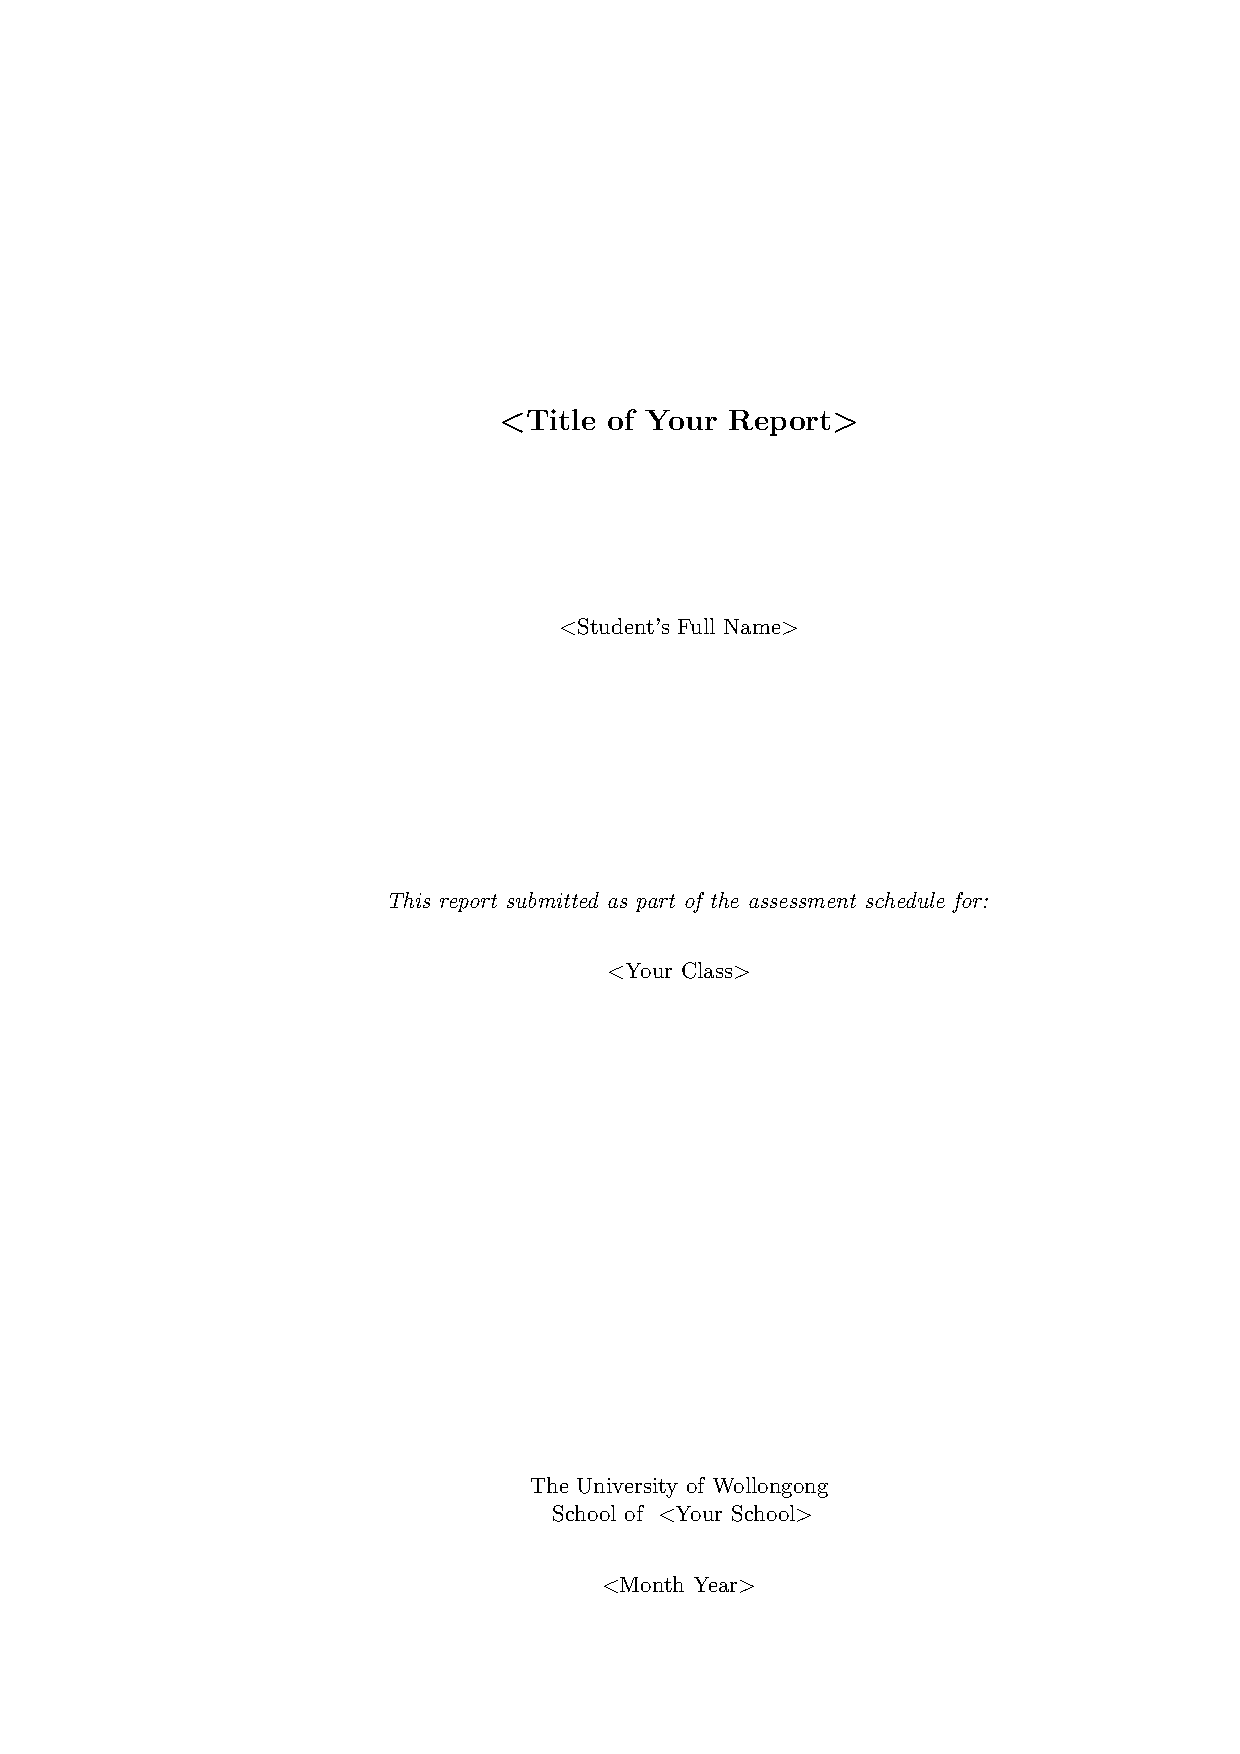
\includepdf{Examples/report.pdf}
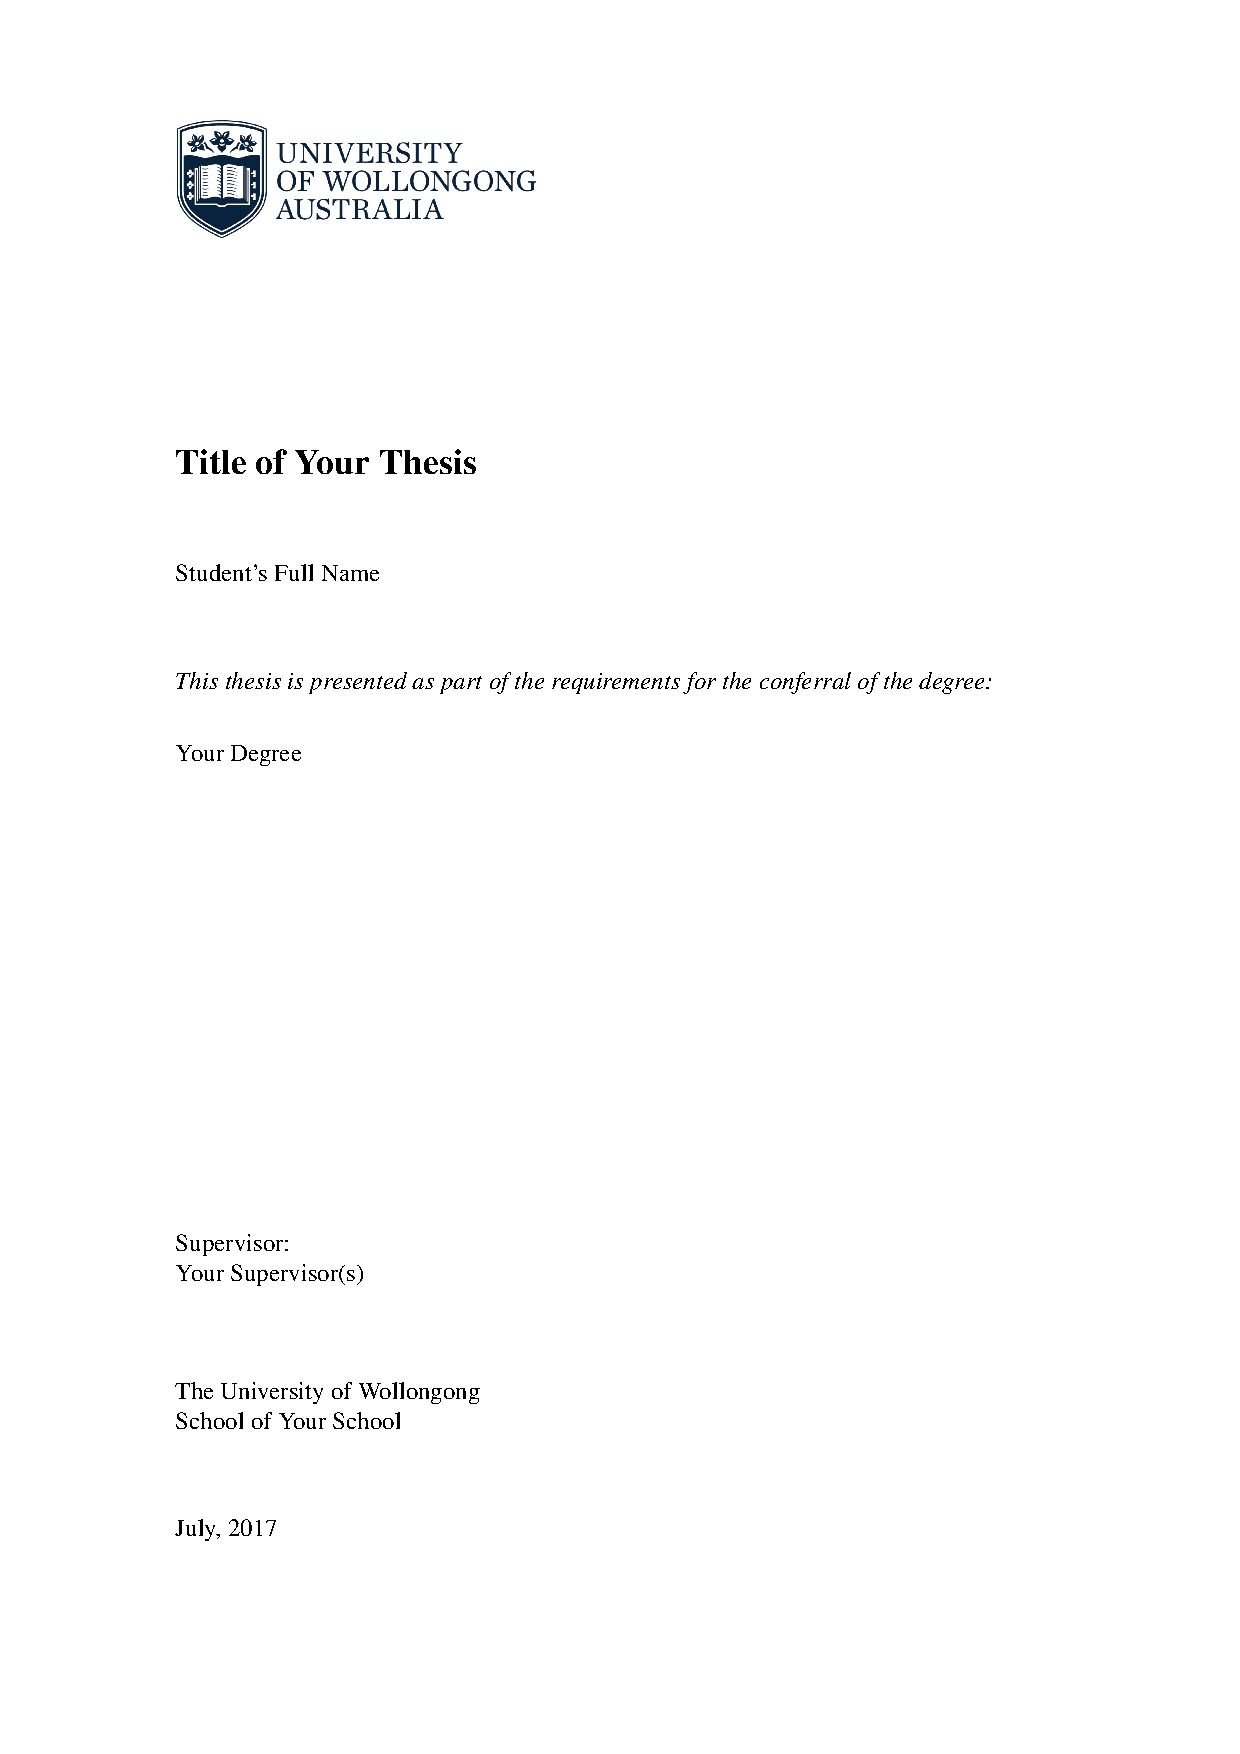
\includepdf{Examples/honours.pdf}
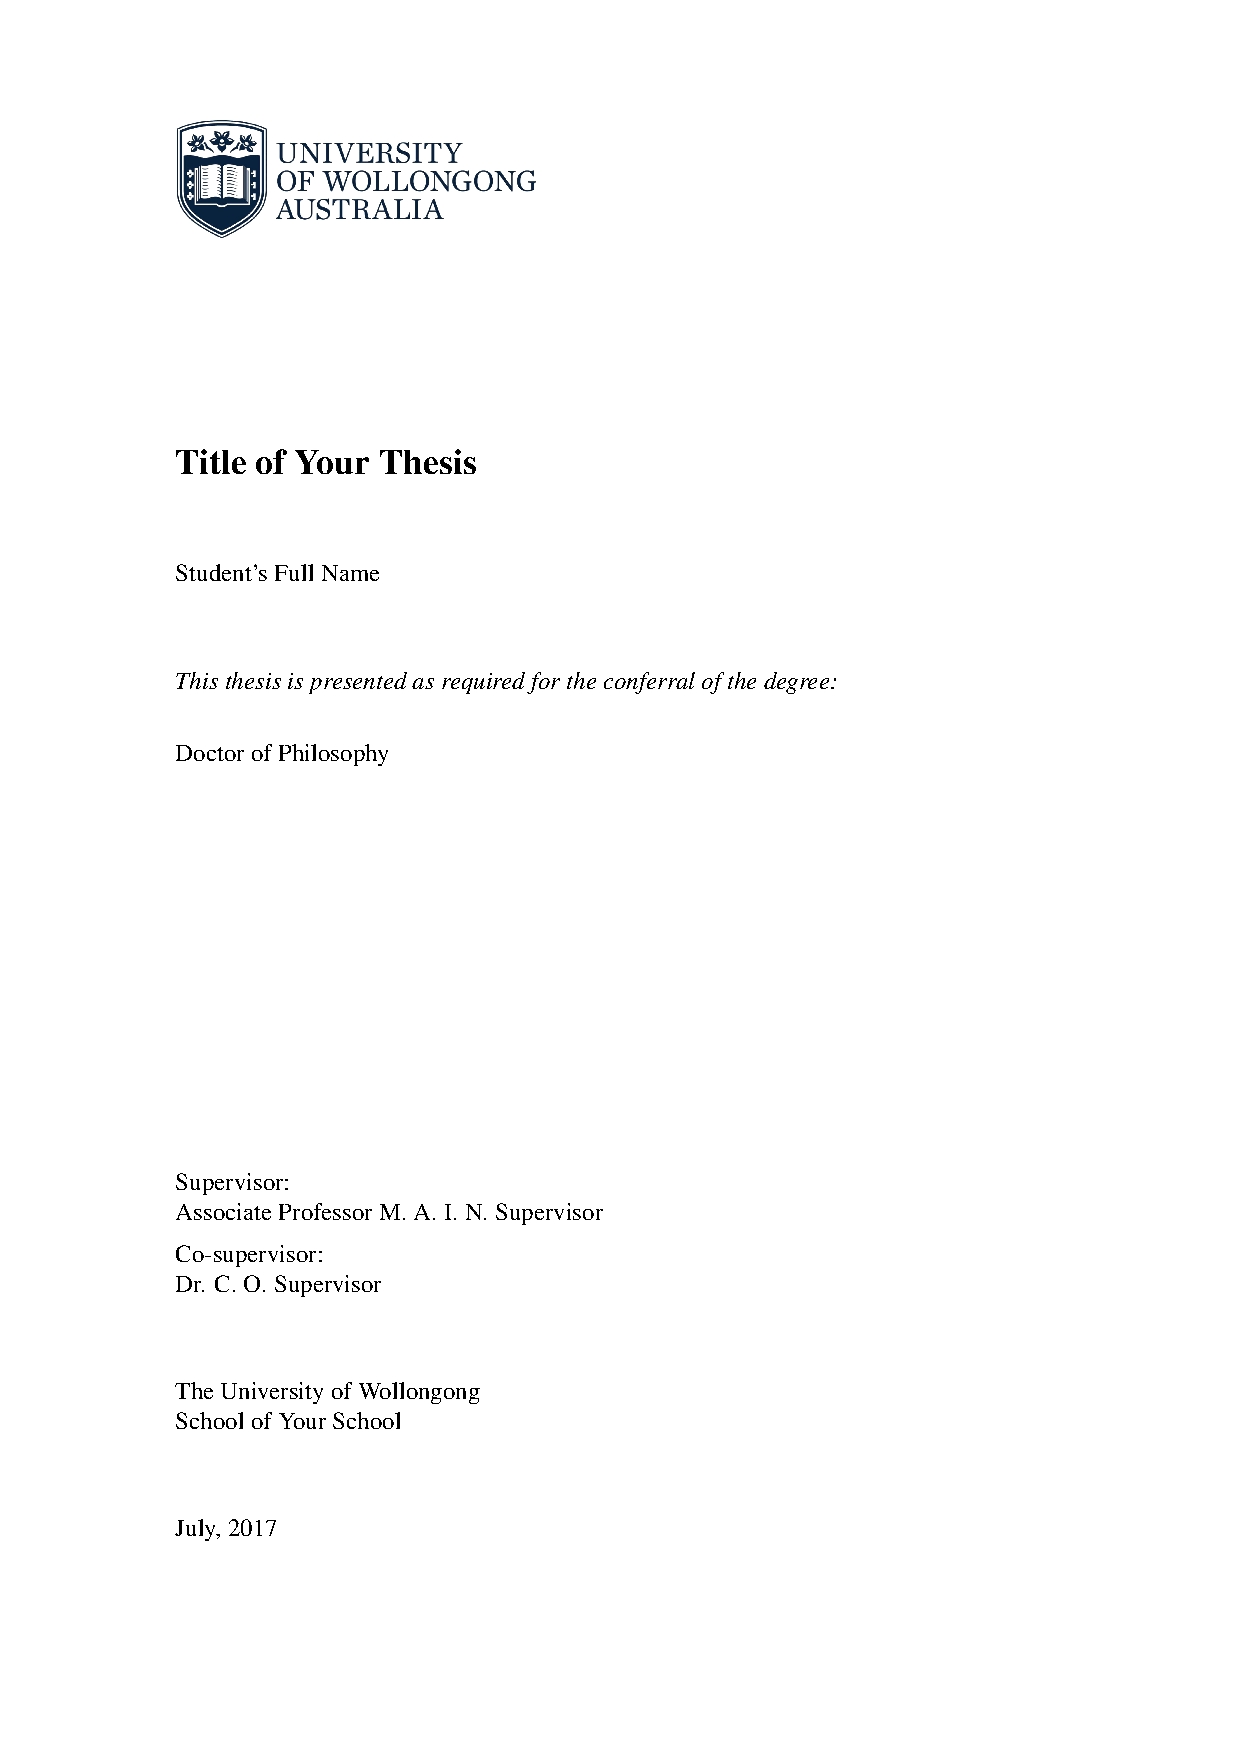
\includepdf{Examples/phd.pdf}

\includepdf{Examples/copyrighttext.pdf}
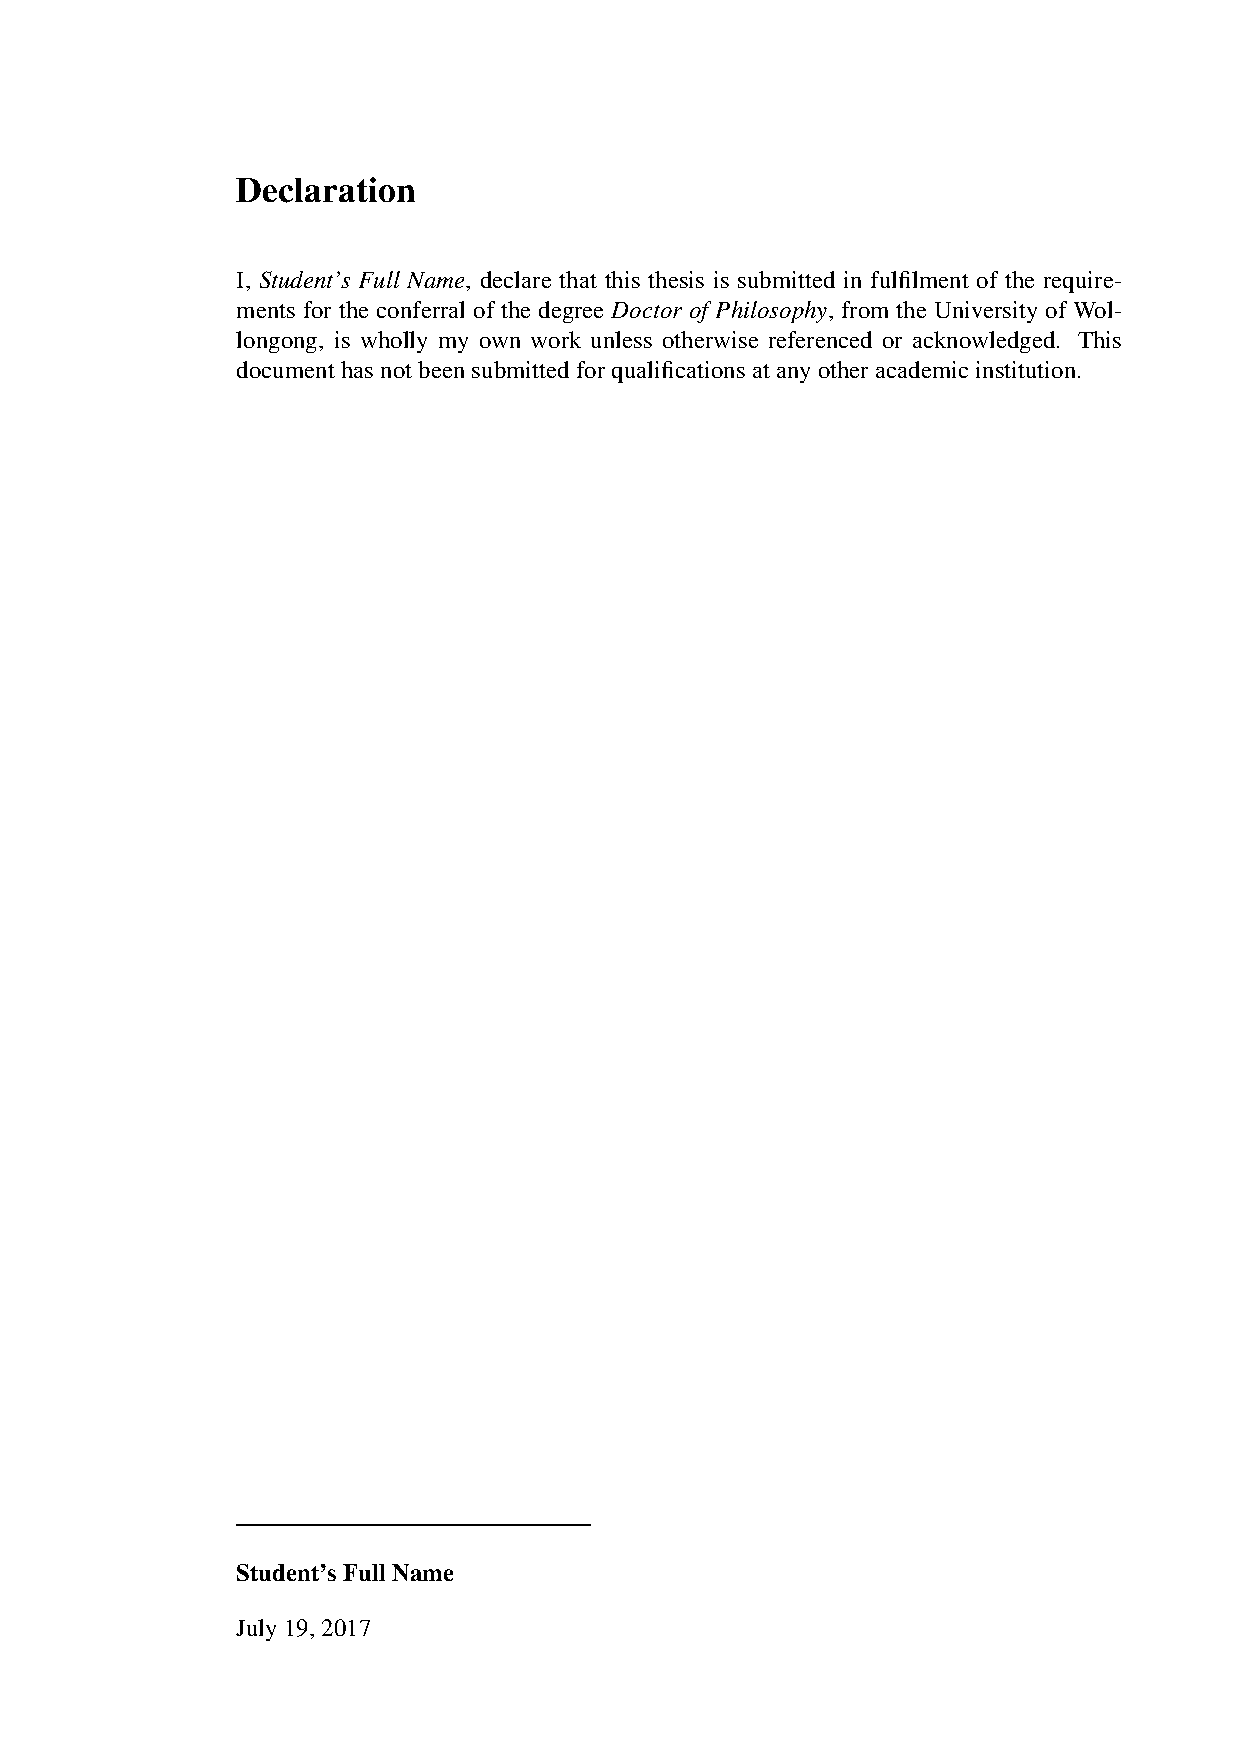
\includepdf{Examples/declaration.pdf}
\end{document}

%Redefinition of \texttt{\textbackslash{}maketitle} to Create a Title Page for a Thesis at the University of Wollongong}}